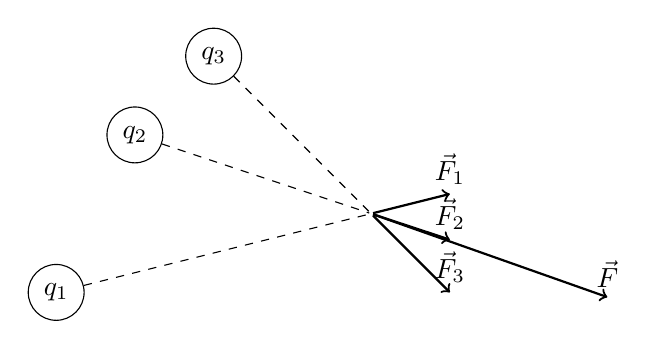
\begin{tikzpicture}
    \path (-3,0) node[draw,circle] (q1) {$q_1$};
    \path (-2,2) node[draw, circle] (q2) {$q_2$};
    \path (-1,3) node[draw, circle] (q3) {$q_3$};
    \path (1,1)  node[inner sep=.1] (p) {};
    \draw [dashed] (q1) -- (p);
    \draw [dashed] (q2) -- (p);
    \draw [dashed] (q3) -- (p);
    \draw [thick,->] (p) -- (2,1.25);
    \draw [thick,->] (p) -- (2,0.67);
    \draw [thick,->] (p) -- (2,0);
    \draw [thick,->] (p) -- (4,-0.06);
    \node[above] at (2,1.25) {$\vec{F}_{1}$};
    \node[above] at (2,0.67) {$\vec{F}_{2}$};
    \node[above] at (2,0) {$\vec{F}_{3}$};
    \node[above] at (4,-0.06) {$\vec{F}$};
\end{tikzpicture}
